\section{Results}
\label{sec:results}

\begin{figure*}[!ht]
 \centering
 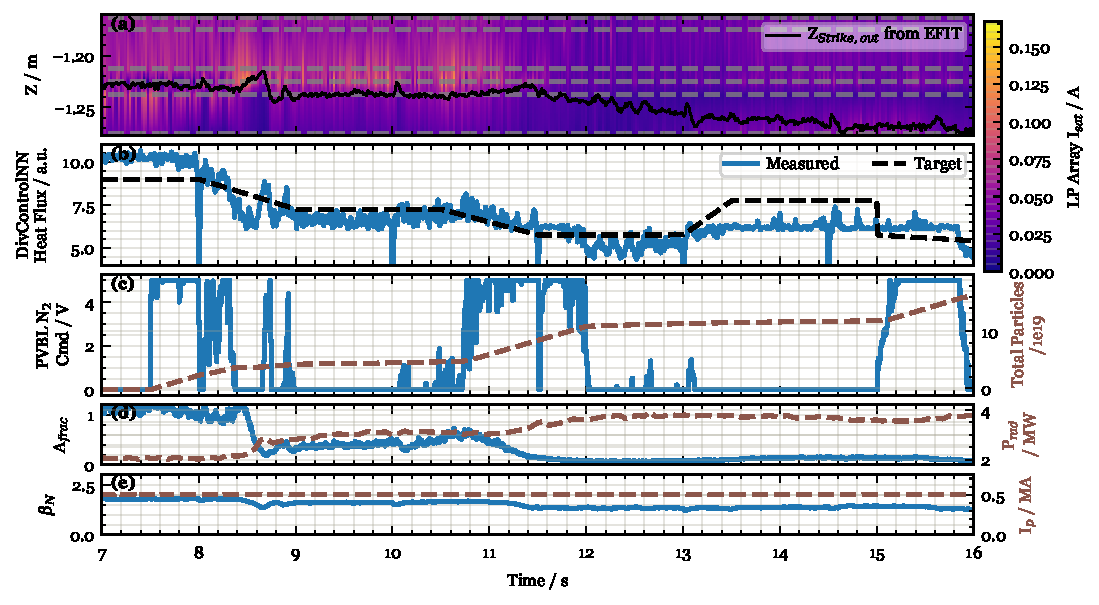
\includegraphics[width=\textwidth]{figures/DetCtrl_2D_36161.pdf}
 \caption{
Detachment control shot \# 36161 using DivControlNN heat flux at outer divertor.
(a) Shows the measured ion saturation current by realtime Langmuir Probe array at locations marked by grey dashed lines.
The data has been interpolated spatially using cubic spline interpolation.
The black curve shows the post-shot calculated strike point position on outer divertor using EFIT.
(b) Shows the heat flux at outer divertor calculated by DivControlNN.
The dashed black line shows the target provided to the controller to follow.
(c) Left axis: Shows the N$_2$ gas command steps sent for system identification.
Right axis: Shows the cummulative N$_2$ gas particles injected into the vessel.
(d) Left axis: Shows the \Afrac calculated from peak value among the Langmuir probe array.
Right axis: Total radiated power measured by \ac{IRVB}.
(e) Left axis: Shows $\beta_n$.
Right axis: Shows the plasma current (I$_p$).
}
 \label{fig:detctrl_sm}
\end{figure*}

\begin{figure}[!h]
 \centering
 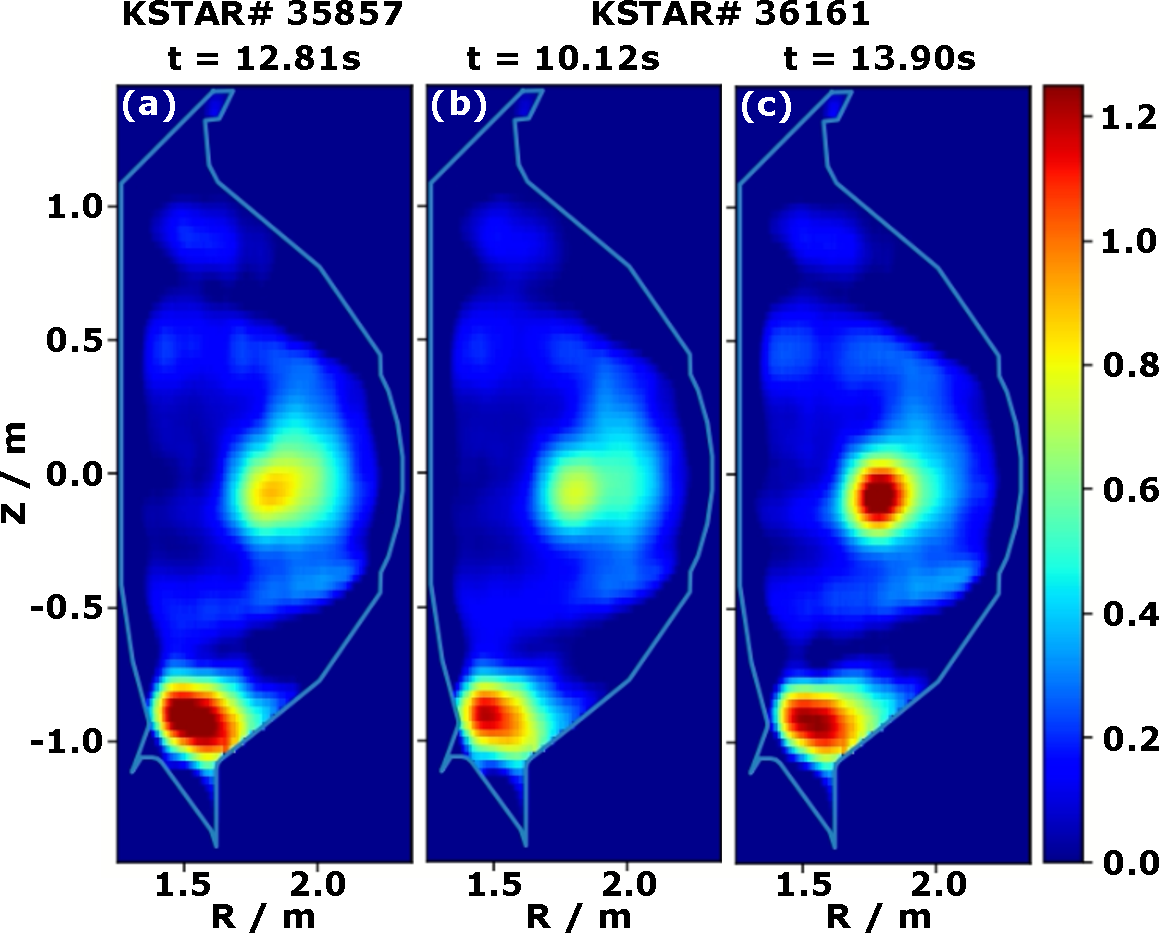
\includegraphics[width=\linewidth]{figures/Prad_2D.pdf}
 \caption{
KSTAR \ac{IRVB} measured radiated power density (a.u.) inverted into 2D cross-section.
(a) KSTAR \# 35857 at 12.81s at the peak of total radiated power.
(b) KSTAR \# 36161 at 10.12s before  the second impulse of gas between 10.8s to 12s.
(c) KSTAR \# 36161 at 13.90 after the last gas impulse.
}
\label{fig:prad_2d}
\end{figure}

Utilizing the controllers tuned in Sec.\ref{sec:sysid}, we attempted detachment control experiments.
First, we used \Afrac{} controller in KSTAR \#35857 with results shown in Fig.\ref{fig:detctrl_afrac}.
As can be seen in Fig.\ref{fig:detctrl_afrac}a, the strike point remained within 12.5~mm of one of the probes of the real-time Langmuir probe array, thus the obtained \Afrac{} signal shown in Fig.\ref{fig:detctrl_afrac}b has error $\lesssim$13\%.
Here, we can see that the controller was successful in closely following the target provided to it completing the pre-programmed shot length to the end.
It is also evident that the aggressive control strategy was reasonable in that it provided a quick response to the initial change in the target value.
There are signs of small decaying oscillations which is a characteristic of a PID loop tuned for faster-than-critical response to reach the target quickly while causing minor decaying oscillations.
While the PID loop can be made less aggressive to critically approach the target, this generally comes at the cost of approximately half the speed with which it is possible to aggressively approach the target while remaining stable.
Here we chose to demonstrate an aggressive strategy but a slower strategy without any oscillations is also possible.
From 8~s to 10~s, it can be seen that the injected N$_2$ was just enough to ramp down the measured \Afrac{} with the same slope.
The accumulated offset from the target eventually caused the integral term to send a brief impulse of nitrogen near 9.8~s and then the controller further converged with the target value.
For the rest of the shot, small nitrogen puffs were required to correct the drifting \Afrac{} and keep it on the target.
The total radiated power from the plasma as measured by KSTAR \ac{IRVB} remained below 3.5~MW ($\approx$65\% of injected power) and as can be seen in Fig.\ref{fig:prad_2d}a (snapshot taken at around the time of maximum radiation), the majority of the radiation was coming from the divertor region and the core region was not losing power through radiation.
\fixme{This statement needs backing; just looking at the heatmap isn't enough. We should have pradcore and praddiv traces to make such a statement. Also, the core literally is losing some power. Just maybe not as much? But the volume is so much bigger that even with lower radiation density, it could be significant.}
This further validated, that \Afrac{} controller strategy first devised in Ref.\cite{Eldon_2022_PPCF} is a viable option for detachment control even with Tungsten divertor in KSTAR.

Since \Afrac{} controller has been demonstrated in the past as well, we decided to utilize the remaining allotted runtime on KSTAR to test the DivControlNN prototype-based controller.
Fig.\ref{fig:detctrl_sm} shows the results from shot \#36161 where we deployed this controller.
An immediate issue was seen with DivControlNN output that the initial heat flux calculation had a different starting value than what we saw in reference shots and system identification shot \#35854 (this shot appeared in figures~\ref{fig:sysid_sm} and \ref{fig:SM_inputs_35854}).
Because of this, when the controller turned on at 7.5~s, the large error resulted in the railing of gas command output which caused too much N$_2$ injected into the system.
While this quickly brought down the measured signal, it also resulted in an overshoot.
In the next ramp-down of the target from 10.5~s to 11.5~s, more impurity was injected as we tuned an aggressive controller.
It can be seen from \Afrac{} in Fig.\ref{fig:detctrl_sm}d that the system reached deep detachment by this point and the ion saturation current measurements (Fig.\ref{fig:detctrl_sm}a) became unreliable beyond 12~s.
In post-analysis of IRVB inverted data as shown in Fig.\ref{fig:prad_2d}, we can see that the core started radiating a lot of power after the last railed impulse of gas input between 10.8~s to 12~s (Fig.\ref{fig:prad_2d}c), whereas \#36161 with DivControlNN heat flux control was similar to \#35857 with \Afrac{} control prior to that (Fig.\ref{fig:prad_2d}b vs Fig.\ref{fig:prad_2d}a).
This would have reduced $P_{SOL}$ (power entering SOL from core) and started to starve the divertor of power, contributing to the failure to follow the rising heat flux target shown in Fig.\ref{fig:detctrl_sm}b between 13 and 15~s.
A stronger driver for the failure to reattach when the heat flux target was increased is probably that the walls were saturated with nitrogen under heavy puffing.
Clean walls are effective at pumping nitrogen as it sticks to them, but heavily saturated walls release nitrogen and can act as a source after gas flow is turned off.
Even if the walls are only a weak or negligible source, they will be much less effective at particle removal and thus nitrogen inventory will not decrease quickly enough to follow a reattaching control target.
Inefficient pumping compared to puffing is a known challenge to control that relies on gas as the primary actuator \cite{Eldon_2017_NF,eldon_2025_ppcf}.
This type of nonlinear response also increases the risk of running an aggressive controller as periods of excess seeding may be difficult to recover from; tuning choices that could be preferable in other contexts are not necessarily the best for detachment control.
\fixme{We may want to be more quantitative about power starvation if we can get calibrated pradcore.}
\fixme{Check for changes in ELMs that might have increased tungsten influx to the core; this peaked on-axis radiation looks like tungsten. Detaching more deeply shouldn't increase tungsten sputtering, but messing with the pedestal could increase penetration of tungsten that's floating around the edge, anyway. Or reduce flushing of tungsten that penetrates.}
% \textcolor{red}{Comment on hysteresis stemming from interaction between core and impurity seeding for divertor management? I'll write something if I can find the right words.}
There is no surprise with the fact that setting target values for an uncalibrated output is not always deterministic and would cause issues as we faced.

Post-shot data analysis discovered further issues in our operation of the DivControlNN model.
The impurity fraction calculation as mentioned in Sec.\ref{sec:control_variables} malfunctioned and sent a constant zero input to the model (see Fig.\ref{fig:SM_inputs_35854}e).
Thus the model was unable to respond directly to large amounts of impurity that were injected into the system and was only relying on data from line-integrated core electron density, input power, and plasma current as real-time inputs.
Despite these limitations, this preliminary test sheds light on the potential of using such a surrogate model-based controller for detachment control in future reactors.

% In the past it has been seen that puffing deuterium is sufficient to attain partial detachment \cite{Loarte_1998_NF, Eldon_2017_NF} when the plasma facing wall is made of carbon.
% Such wall can create an intrinsic source of carbon due to sputtering due to ELMS.
% Such intrinsic impurity population can drive detachment through increased electron density as radiated power due to impurity is given by $P_{rad}=n_e n_Z L_Z(T_e)$ where $n_e$ is electron density, $n_Z$ is ion density, and $L_Z(T_e)$ is the radiative loss function for the impurity ion.
% Thus, in the presence of some intrinsic impurity
% \textcolor{red}{No, not deuterium alone. Deuterium \emph{puffing} alone can do it, if there's a carbon wall to sputter to make a carbon source to go with the deuterium puff. KSTAR still has a carbon main wall that could do it. Also, $P_{rad}=n_e n_Z L_Z(T_e)$, so changing $n_e$ when you have some background impurity will do it. So yes, puffing deuterium in the presence of some fixed impurity population will drive detachment, even if the D2 doesn't trigger any additional sputtering related impurity influx. The ELMs will have knocked carbon off the main chamber wall. Then increasing deuterium density in the divertor will increase $n_e$ and therefore $P_{rad}$. Be precise about these things. The results you quoted were from carbon-walled devices. Not for this paper per se but for fun, check ASDEX Upgrade results to see if detachment can be achieved with D2 only puffing in full tungsten.}
% This might be the case with shot \#36161, that the model inference with zero impurity fraction input still reported a decrease in estimated heat flux as the electron density input increased with N$_2$ puffing.
% % \textcolor{red}{Did they put background carbon in? Although the seeded impurity (neon I think in that version of DivControlNN) may have been 0, the intrinsic impurity might not have been.} No there was no intrinsic impurity in the sims
% The only other changeable input, input power, mostly remained constant during flat top of the shot.
% However, as the amount of total puffed N$_2$ increased, the pure deuterium plasma case from which the model must be infering the heat flux would deviate and thus the control is not very good beyond 11s.
% \textcolor{red}{I don't think this logic holds up. The control variable might not correlate well with reality if changes in impurity fraction become too large, but if it still responds similarly to the control actuator, that shouldn't be a barrier to control. It's not clear that you can blame deficiencies in control performance on this.}
% Despite these limitations, this preliminary test sheds light on the potential of using such a surrogate model-based controller for detachment control in future reactors.
